\chapter{Export}\label{export}
\section{Aktivitäten}\label{export:aktivitaeten}
\begin{figure}[!h]
	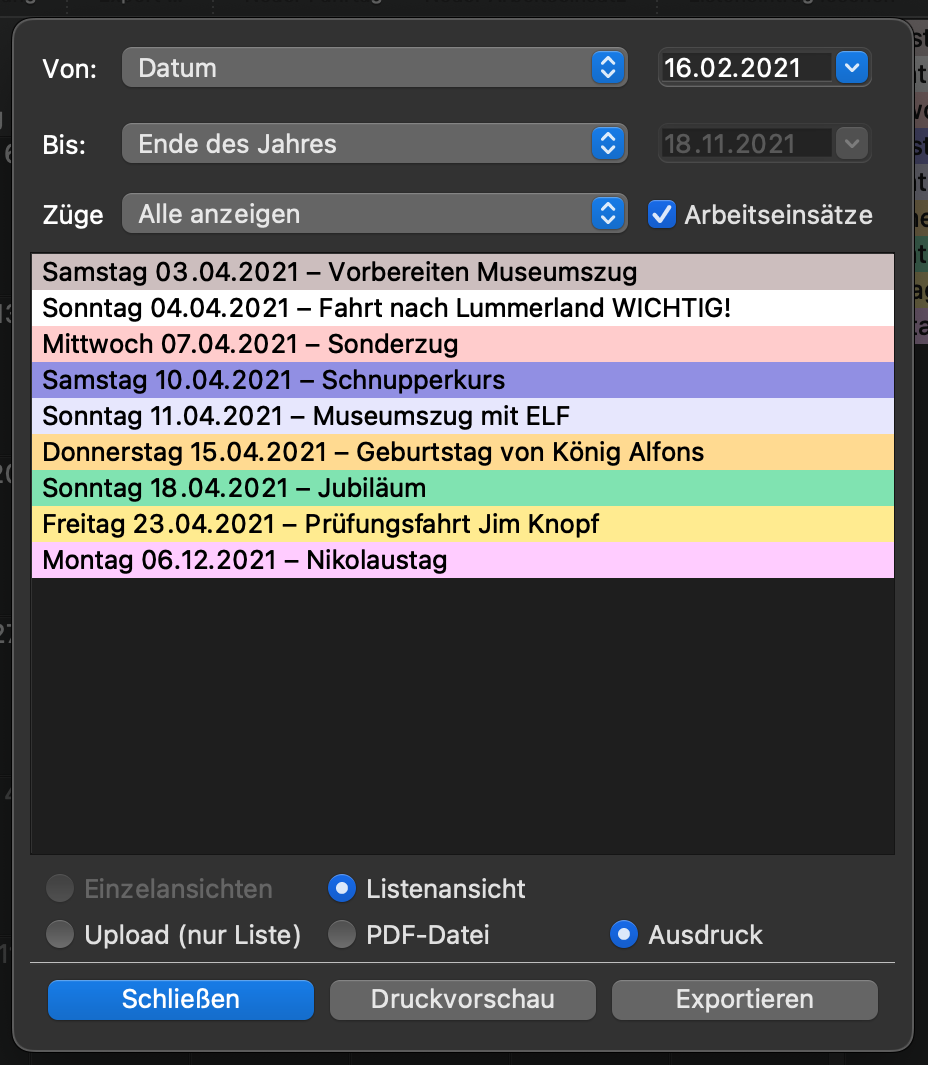
\includegraphics[width=\textwidth]{img/export}
	\caption{Der Exportdialog im Hauptfenster.}
	\label{fig:export:aktivitaeten}
\end{figure}
Im Startfenster öffnet sich über den Knopf \emph{Exportieren \dots} der Dialog in Abbildung~\ref{fig:export:aktivitaeten}.
Dort kann mit den beiden Auswahlfeldern am oberen Ende eine zeitliche Beschränkung der Aktivitäten angegeben werden.
Mit dem darunterlegenden Auswahlfeld, kann bestimmt werden, welche Art von Fahrtag exportiert werden soll (z.B.\ nur Nikolausszüge).
Auch kann hier ausgewählt werden, ob die Arbeitseinsätze nicht ausgegeben werden sollen.

Alle Aktivitäten, die in der Liste angezeigt werden, werden bei einem Export per Listenansicht ausgegeben.

Um eine Einzelansicht einzelner Aktivitäten auszugeben, müssen Sie die entsprechenden Aktivitäten in der Liste durch einen Klick auf das Element auswählen bzw.\ abwählen.

Um die entsprechenden Ansichten zu generieren, setzen Sie den Haken an den entsprechenden Auswahlkästen.
Ebenso können Sie hier bestimmen, ob die Ausgabe als PDF-Datei auf den zuvor konfigurierten Webserver hochgeladen (Kapitel~\ref{upload}),
als PDF-Datei gespeichert oder auf einem Drucker gedruckt werden soll.
Für den Export in eine PDF-Datei wird ein Fenster geöffnet, in dem Sie den Speicherort auswählen können.
Sollten Sie die Dokumente drucken wollen,
öffnet sich das Drucker-Fenster Ihres Betriebssystems,
in dem Sie weitere Einstellungen vornehmen können (Papierformat, Ausrichtung, \dots).

Diese Einzelansicht kann für jede Aktivität auch im entsprechenden Fenster direkt generiert und als PFD gespeichert oder gedruckt werden.


\section{Reservierungen}
Ein Fahrtag bietet noch eine weitere Methode Informationen zu exportieren.
Diese Funktion wird vor allem bei Nikolausfahrten benötigt.
Denn bei diesem Ausgabeformat werden viele Reservierungen übersichtlich nach Wagen sortiert ausgegeben.
Diese Funktion ist insbesodnere bei Nikolausfahrten wichtig, da dort keine Reservierungen in der Einzelansicht ausgegeben werden.

Diese Funktion ist für jeden Fahrtag über das Menü "`Fahrtag"' erreichbar.
Es gibt die Möglichkeit das Dokument entweder als PDF zu speichern oder auf einem Drucker zu drucken.

Das exportierte Dokument enthält folgende Informationen zu einer Reservierung: Name, Anzahl Sitzplätze, Sitzplätze, Kommentare/Bemerkungen sowie den Zustieg, sofern er verschieden von Ottweiler ist.



\section{Einsatzzeiten des Personals}
Es stehen folgende Übersichten zur Verfügung, die alle über das Menü "`Exportieren"' im Fenster des Personalmanagements aufgerufen werden können:
\begin{description}
  \item[Gesamtübersicht des Personals]
  Alle in der Tabelle angezeigten Informationen werden in der angegebenen Sortierung ausgegeben.
  Diese Ausgabemöglichkeit ist auch über die zwei Knöpfe in der Gesamtübersicht verfügbar.
  \item[Einzelansicht der aktuellen Person]
  Es werden nur die Einsatzzeiten der aktuell in der Einzelansicht angezeigten Person ausgegeben.
  Dieses Format enthält die Aktivitäten, die Einsatzzeiten und Mindeststunden für die jeweilige Person.
  Ebenso wird die betriebliche Ausbildung (sofern vorhanden und Tauglichkeit gegeben) und die Entfernung zum Bahnhof angegeben.
  \item[Einzelansichten des Personals]
  Erstellt eine Übersciht wie unter Punkt zwei für jede in der Liste/Tabelle angezeigt Person nach Name sortiert.
  Alle Übersichten werden in einer Datei zusammengefasst und durch eine Übersicht ergänzt, welche die Summe aller geleisteten Stunden umfasst.
  Dort sind auch die Mindeststunden der einzelnen Kategorien angegeben.
\end{description}



\section{Mitglieder}
Über das Export-Menü im Fenster für das Personalmanagement kann eine umfassende Mitgliederliste ausgegeben werden.
In dieser Liste sind alle Personen enthalten, die im System registriert sind.
Ausgegeben werden dabei alle Personenbezogenen Daten, die im Programm verwaltet werden.
Einsatzzeiten und geleistete Stunden sind in diesen Ansichten nicht enthalten.

Ebenso können diese Daten auch als CSV-Datei ausgegeben werden, um sie in anderen Programmen weiter zu verarbeiten.
